\frame{
\frametitle{Klassenstruktur}
    \begin{block}{Struktur}
    \begin{itemize}
        \item Wichtigsten \textbf{Optionen} auf einen Blick
        \item Anbindung an Datenbanken für \textbf{Email und Kalender}
        \item Einstellung für \textbf{Benachrichtigungen}
    \end{itemize}
    \begin{figure}
    		\centering
    		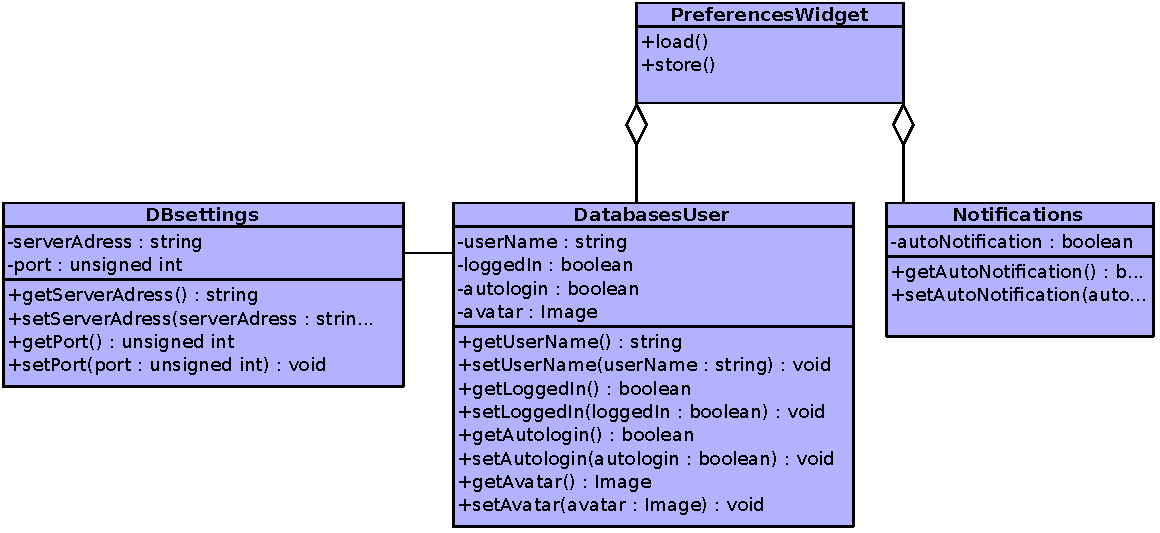
\includegraphics[width=0.6\textwidth]{../grafiken/PreferencesWidget_Class.pdf}
    		\caption{Klassenstruktur für das Optionsmenü.}
    \end{figure}
        
    \end{block}

}